\chapter*{Dodatak: Prikaz aktivnosti grupe}
		\addcontentsline{toc}{chapter}{Dodatak: Prikaz aktivnosti grupe}
		
		\section*{Dnevnik sastajanja}
		

		\begin{packed_enum}
			\item  sastanak
			
			\item[] \begin{packed_item}
				\item Datum: 19. listopada 2023.
				\item Prisustvovali: E.Habek, M.Plavec, A.Dautović, L.Grubišin, A.Đurđević, M.Magat, A.Stanković
				\item Teme sastanka:
				\begin{packed_item}
					\item procjena vještina i motivacija članova tima
					\item izmijena ideja o načinu provedbe projekta
					\item upoznavanje
					\item odabir tehnologija
				\end{packed_item}
			\end{packed_item}
			
			\item  sastanak
			\item[] \begin{packed_item}
				\item Datum: 24. listopada 2023.
				\item Prisustvovali: E.Habek, M.Plavec, A.Dautović, L.Grubišin, A.Đurđević, M.Magat, A.Stanković
				\item Teme sastanka:
				\begin{packed_item}
					\item razrada projekta
					\item zajedničko iznošenje ideja za obrasce uporabe
					\item podjela posla za pisanje dokumentacije za naredni tjedan
					\item međusobno pomaganje i dijeljenje znanja o Gitu
				\end{packed_item}
			\end{packed_item}
			
			\item  sastanak
			\item[] \begin{packed_item}
				\item Datum: 31. listopada 2023.
				\item Prisustvovali: E.Habek, M.Plavec, A.Dautović, L.Grubišin, A.Đurđević, M.Magat, A.Stanković
				\item Teme sastanka:
				\begin{packed_item}
					\item skica baze podataka
					\item skica grafičkog sučelja
					\item skica ruta
					\item razrješiti nedoumice
				\end{packed_item}
			\end{packed_item}

			\item  sastanak
			\item[] \begin{packed_item}
				\item Datum: 7. studenog 2023.
				\item Prisustvovali: E.Habek, M.Plavec, A.Dautović, L.Grubišin, A.Đurđević, M.Magat, A.Stanković
				\item Teme sastanka:
				\begin{packed_item}
					\item iznošenje svojih problema te zajedničko pronalaženje rješenja
					\item diskutiranje o specifičnim svojstvima baze podataka
				\end{packed_item}
			\end{packed_item}

			\item  sastanak
			\item[] \begin{packed_item}
				\item Datum: 14. studenog 2023.
				\item Prisustvovali: E.Habek, M.Plavec, A.Dautović, L.Grubišin, A.Đurđević, M.Magat, A.Stanković
				\item Teme sastanka:
				\begin{packed_item}
					\item programeri pokazuju i objašnjavaju ono što su učinili
					\item diskutiranje kako ćemo deployati
				\end{packed_item}
			\end{packed_item}

			\item  sastanak
			\item[] \begin{packed_item}
				\item Datum: 19. prosinca 2023.
				\item Prisustvovali: E.Habek, M.Plavec, A.Dautović, L.Grubišin, A.Đurđević, M.Magat, A.Stanković
				\item Teme sastanka:
				\begin{packed_item}
					\item dijeljenje trenutnog napretka
					\item dogovor o daljnjem ophođenju preko zimskih praznika
				\end{packed_item}
			\end{packed_item}

			\item  sastanak
			\item[] \begin{packed_item}
				\item Datum: 4. siječnja 2024.
				\item Prisustvovali: E.Habek, M.Plavec, A.Dautović, L.Grubišin, A.Đurđević, M.Magat, A.Stanković
				\item Teme sastanka:
				\begin{packed_item}
					\item dijeljenje trenutnog napretka
					\item iznošenje problema i razmišljanje o rješenjima
				\end{packed_item}
			\end{packed_item}

			\item  sastanak
			\item[] \begin{packed_item}
				\item Datum: 9. siječnja 2024.
				\item Prisustvovali: E.Habek, M.Plavec, A.Dautović, L.Grubišin, A.Đurđević, M.Magat, A.Stanković
				\item Teme sastanka:
				\begin{packed_item}
					\item pokazivanje programske potpore
				\end{packed_item}
			\end{packed_item}

			\item  sastanak
			\item[] \begin{packed_item}
				\item Datum: 16. siječnja 2024.
				\item Prisustvovali: E.Habek, M.Plavec, A.Dautović, L.Grubišin, A.Đurđević, M.Magat, A.Stanković
				\item Teme sastanka:
				\begin{packed_item}
					\item dogovoravanje puštanje u pogon
				\end{packed_item}
			\end{packed_item}
			%
			
		\end{packed_enum}
		
		\eject
		\section*{Tablica aktivnosti}
		
			\begin{longtblr}[
					label=none,
				]{
					vlines,hlines,
					width = \textwidth,
					colspec={X[7, l]X[1, c]X[1, c]X[1, c]X[1, c]X[1, c]X[1, c]X[1, c]}, 
					vline{1} = {1}{text=\clap{}},
					hline{1} = {1}{text=\clap{}},
					rowhead = 1,
				} 
			
				\SetCell[c=1]{c}{} & \SetCell[c=1]{c}{\rotatebox{90}{\textbf{Eloise Habek }}} & \SetCell[c=1]{c}{\rotatebox{90}{\textbf{Anabel Dautović }}} &	\SetCell[c=1]{c}{\rotatebox{90}{\textbf{Mateo Plavec }}} & \SetCell[c=1]{c}{\rotatebox{90}{\textbf{Luka Grubišin }}} &	\SetCell[c=1]{c}{\rotatebox{90}{\textbf{Alan Đurđević }}} & \SetCell[c=1]{c}{\rotatebox{90}{\textbf{Matej Magat }}} &	\SetCell[c=1]{c}{\rotatebox{90}{\textbf{Andrej Stanković }}} \\
				Upravljanje projektom 		& 7 &  &  &  &  &  & \\
				Opis projektnog zadatka 	&  &  &  & 5 &  &  & \\
				
				Funkcionalni zahtjevi       & 3 &  &  & 5 &  &  &  \\
				Opis pojedinih obrazaca 	& 5 &  & 1 &  &  & 2 &  \\
				Dijagram obrazaca 			& 5 &  &  &  &  &  &  \\ 
				Sekvencijski dijagrami 		&  &  &  &  &  &  &  4\\ 
				Opis ostalih zahtjeva 		&  &  &  & 1  &  &  &  \\ 

				Arhitektura i dizajn sustava	 &  &  &  & 2  &  &  &  \\ 
				Baza podataka				&  & 8 &  &  &  &  &   \\
				Dijagram razreda 			&  & 10 &  &  &  &  &   \\
				Dijagram stanja				& 6 &  &  &  &  &  &  \\ 
				Dijagram aktivnosti 		&  &  &  & 2 &  &  &  \\ 
				Dijagram komponenti			&  & 10 & 1 &  &  &  &  \\ 
				Korištene tehnologije i alati 		& 2 &  &  &  &  &  &  \\ 
				Ispitivanje programskog rješenja 	&  &  &  & 11 &  &  &  \\ 
				Dijagram razmještaja			&  &  &  & 1 &  &  &  \\ 
				Upute za puštanje u pogon 		&  &  &  & 2 &  & 1 &  \\  
				Dnevnik sastajanja 			& 1 &  &  &  &  &  &  \\ 
				Zaključak i budući rad 		& 1 & 3 &  &  &  &  &  \\  
				Popis literature 			& 1 &  &  &  &  &  &  \\  
				&  &  &  &  &  &  &  \\ \hline 
				\textit{Postavljanje programske potpore} 			& 1 &  & 3 & 2 & 2  &  &  \\
				\textit{GitHub admin} 			&  &  & 4 &  &  &  &  \\
				\textit{Proučavanje backend i frontend tehnologija} 	&  &  &  & 1 & 8 & 6 & 2\\ 
				\textit{Dizajn aplikacije} 				&  &  &  &  &  &  &  20\\  
				\textit{Izrada frontenda} 				&  &  &  &  &  & 29 & 2\\  
				\textit{izrada baze podataka} 		 			&  &  & 1 &  &  &  & \\  
				\textit{spajanje s bazom podataka} 							&  &  &  &  &  &  &  \\ 
				\textit{Izrada backenda} 							&  &  & 29 &  & 20 & 3 &  \\  
				\textit{deploy} 							& 1 &  & 4 &  &  & 1 &  \\
				\textit{provjera dokumentacije} 							& 6 &  & 1 & 1 &  &  &  \\
				\textit{izrada sustava poruka} 							&  &  &  &  & 5 &  &  \\	
				\textit{traženje video API} 							& 2 &  &  &  &  &  &  \\
				\textit{izrada sustava pratitelja} 							& 2 &  &  &  & 5 &  &  \\
				\textit{testiranje} 							&  &  & 3 &  &  &  &  \\
				\textit{izrada prezentacije} 							&  & 3 &  &  &  &  &  \\
			\end{longtblr}
					
					
		\eject
		\section*{Dijagrami pregleda promjena}
		

		\begin{figure}[h]
			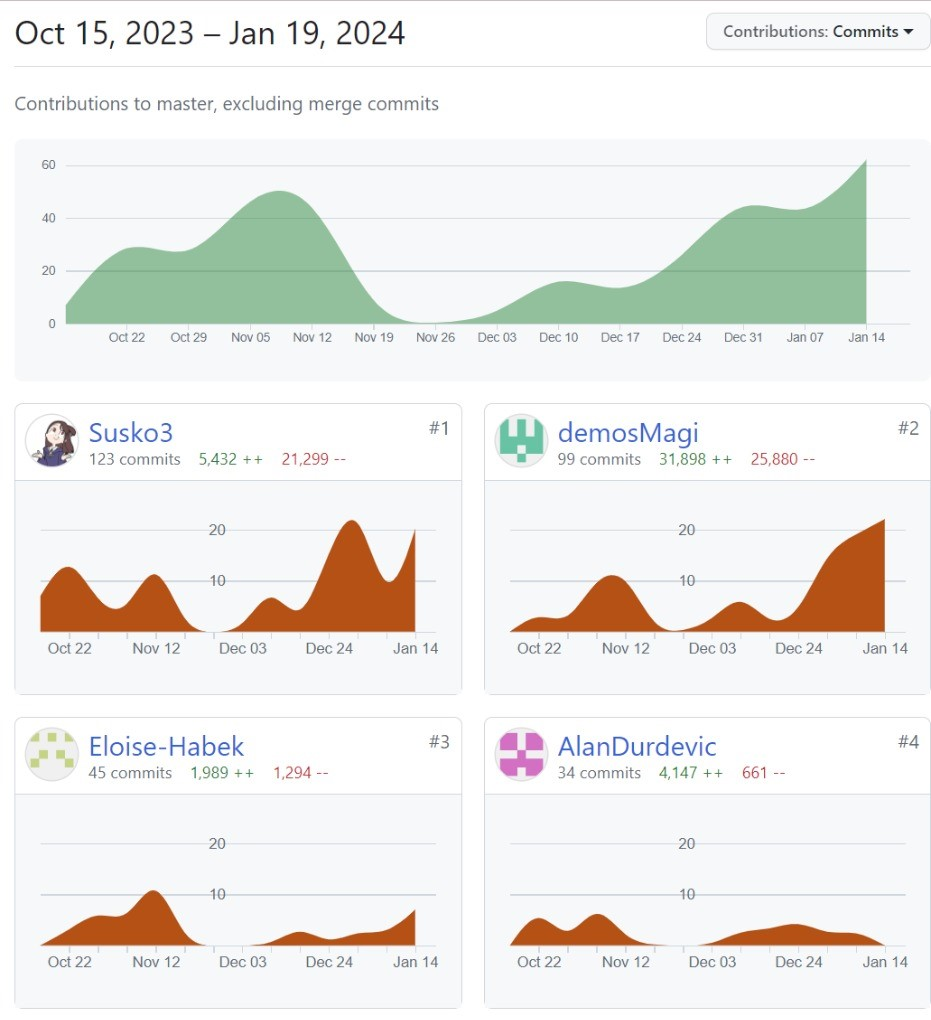
\includegraphics[scale=0.55]{slike/dijagram_promjena1.jpeg}
			\centering
			\caption{Dijagram komponenti - prvi dio}
			\label{fig:dijagram_promjena}
		\end{figure}

		\begin{figure}[h]
			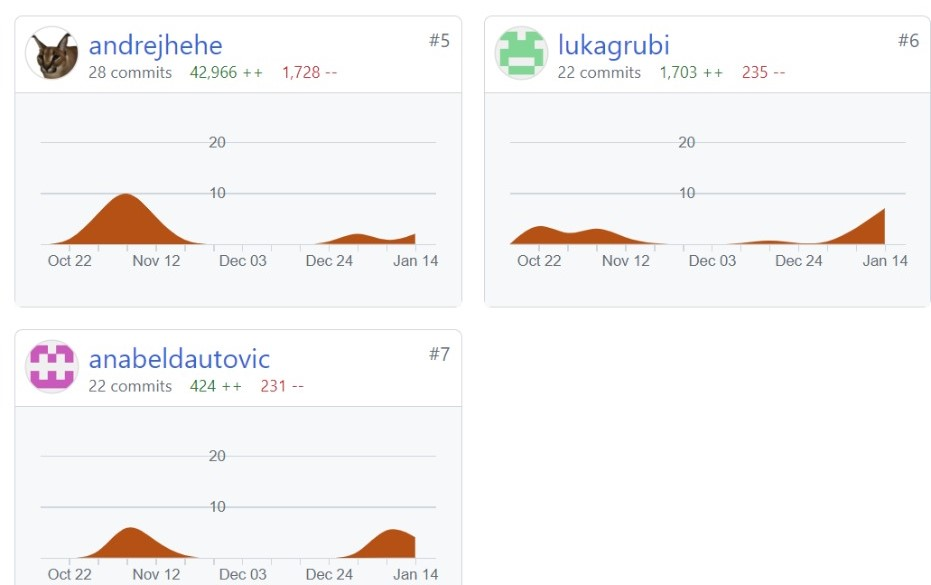
\includegraphics[scale=0.6]{slike/dijagram_promjena2.jpeg}
			\centering
			\caption{Dijagram komponenti - drugi dio}
			\label{fig:dijagram_promjena}
		\end{figure}

		\eject
